% ch1.tex
% This work is licensed under the Creative Commons Attribution-Noncommercial-Share Alike 3.0 New Zealand License.
% To view a copy of this license, visit http://creativecommons.org/licenses/by-nc-sa/3.0/nz
% or send a letter to Creative Commons, 171 Second Street, Suite 300, San Francisco, California, 94105, USA.


\chapter{Nem todas cobras irão te morder}\label{ch:notallsnakeswillsquishyou}

Há possibilidade de que este livro tenha sido lhe dado em seu aniversário, ou possivelmente no Natal. Tia Amélia lhe daria um par de meias duas vezes maior que o seu pé (e que mesmo se servisse, você não gostaria de usar). Mas ao invés disso, ela ouviu alguém falando sobre a versão impressa deste livro e logo lembrou que você tinha um daqueles compu-alguma-coisa, que inclusive tentou ensiná-la a usar uma vez, no último Natal (até que ela começasse a tentar falar com o mouse), e pediu-lhe para que imprimisse mais uma cópia. Seja grato por não ter ganho aquele velho par de meias.

Espero que você não esteja tão decepcionado, por eu surgir de um papel de presentes reciclado, ao invés disso. Um não-tão-falante (ok, um nada-falante) livro, com um título aparentemente ameaçador na capa ``Aprendendo$\ldots$''.
Mas espere um momento para pensar em como eu me sinto. Se você fosse o personagem daquela novela sobre magos que estão na prateleira de livros do seu quarto, eu possivelmente teria dentes… ou até olhos. Eu poderia mover figuras dentro de mim, ou ser capaz de fazer sons fantasmagóricos enquanto você folheia minhas páginas. Mas pelo contrário, eu sou impresso em folhas de papel A4 com algumas orelhas, ou quem sabe grampeados, dentro de uma pasta. Como eu saberia---Eu não tenho olhos.
\\
\\
\emph{Eu daria qualquer coisa por alguns belos e afiados dentes$\ldots$}
\\
\\
Porém isso não é tão ruim quanto parece. Mesmo que eu não possa falar... ou morder os seus dedos enquanto não está olhando... Eu posso lhe dizer um pouquinho como os computadores funcionam. Nada da parte física, com fios, chips, cabos e outros dispositivos que, mais do que provável, lhe dariam choque antes mesmo que o tocassem (então, não!!)---mas as coisas escondidas que rodam entre esses fios, chips de computador, cabos e bits, que fazem o seu computador ter alguma utilidade.

\begin{wrapfigure}{r}{0.5\textwidth}
  \begin{center}
\includegraphics*[width=70mm]{eps/electrocute.eps}
  \end{center}
\end{wrapfigure}

É um pouco como os pensamentos rodando dentro da sua cabeça. Se você não tivesse pensamentos, você estaria sentado no chão do seu quarto, olhando vagarosamente para a porta e babando sobre a sua camiseta. Sem os \emph{programas}, os computadores serviriam apenas para apoiar portas---e mesmo assim ainda não seriam muito úteis, pois você ainda tropeçaria sobre eles durante a noite. E convenhamos que, não há nada pior que tropeçar no escuro e bater o dedinho do pé.
\\
\\
\emph{Eu sou apenas um livro e eu sei disso.}
\\
\\
Sua família pode ter um Playstation, Xbox ou Wii na sala----eles não teriam muito uso sem os programas (jogos) para fazê-los funcionar. Seu aparelho de DVD, possivelmente sua geladeira e seu carro, todos usam programas de computador que os tornam mais prestativos do que seriam. Seu aparelho de DVD tem programas que ajudam-o a escolher o que quer assistir no DVD; sua geladeira pode ter um simples programa que o ajuda a economizar energia elétrica, e mesmo assim mantém a comida conservada; seu carro pode ter um computador, que possui um programa, que alerta o motorista sobre uma possível colisão.\\
Se você souber como escrever programas de computador, você pode fazer todos tipos de coisas úteis. Quem sabe escrever seus próprios jogos. Criar web sites que realmente façam algo, não apenas deixá-los com um visual colorido. Ser capaz de programar o ajudaria até com o seu dever de casa.\\
\\
Como dito, vamos para algo um pouco mais interessante.

\section{Um pouco sobre linguagens}

Assim como os humanos, certamente as baleias, possivelmente os golfinhos, e talvez alguns pais (embora isso seja discutível), computadores tem sua própria linguagem. Atualmente, como os humanos, eles tem até mais de uma linguagem. Praticamente há uma linguagem para cada letra do alfabeto. A, B, C, D e E não são apenas letras, mas também linguagens de programação (que provam que adultos não tem imaginação, e deveriam ter lido um dicionário, ou ao menos uma enciclopédia, antes de nomear algo).

Há linguagens de programação com nomes de pessoas, nomeadas usando simples acrônimos (a primeira letra de uma série de palavras), e apenas algumas nomeadas após um programa de TV. Ah, e se você adicionar alguns sinais de adição, ou sustenidos (+, \#) após algumas das letras que mencionei---você terá mais algumas linguagens de programação. Tornando as coisas piores, algumas linguagens de programação são praticamente a mesma coisa, diferenciando-se levemente.
\\
\\
\emph{O que eu te disse?  Sem imaginação!}
\\
\\
Felizmente, muitas dessas linguagens caíram em desuso, ou sumiram completamente; mas a lista de diferentes formas que você pode `falar' com o computador continua preocupantemente grande. Irei discutir apenas uma delas--caso contrário nem mesmo teriamos começado.
\\
Seria mais produtivo sentar-se em seu quarto e babar sobre a sua camiseta$\ldots$

\section{A Ordem das Não-venenosas \\Serpentes Constritoras$\ldots$}

$\ldots$ou Pythons (Pítons em português), mais especificamente.

Além de ser uma cobra, Python\index{Python} também é uma linguagem de programação. Porém, não foi nomeada com o nome de um réptil sem patas; mas é uma das linguagens de programação nomeadas após um programa de TV. Monty Python foi um popular programa humorístico de TV britânico, durante a década de 70 (e continua popular até hoje), que você deve ter uma certa idade para achar engraçado. Qualquer um abaixo dessa idade$\ldots$ digamos 12$\ldots$ irá se perguntar do que se trata\footnote{Exceto a dança-do-peixe-na-cara. Que é engraçado independente da sua idade.}.

Existe uma série de coisas sobre Python (a linguagem de programação, não a cobra, nem o programa de TV) que a fazem extremamente útil quando você está aprendendo a programar. Para nós, no momento, o motivo mais importante é que você pode começar a fazer as coisas muito rapidamente.

Esta é a parte que você espera que a sua Mãe, Pai (ou quem estiver responsável pelo computador), tenha lido o começo do livro, rotulado ``Um recado aos Pais''.

\noindent
Existe um bom modo de saber se eles realmente leram:

\begin{WINDOWS}
Click on the Start button at the bottom left of the screen, click on `All Programs' (which has a green triangle next to it), and hopefully in the list of programs you should see `Python 2.5' (or something like it).  Figure~\ref{fig1} shows you what you should be looking for. Click on `Python (command line)' and you should see something like Figure~\ref{fig2}.

\begin{figure}
\begin{center}
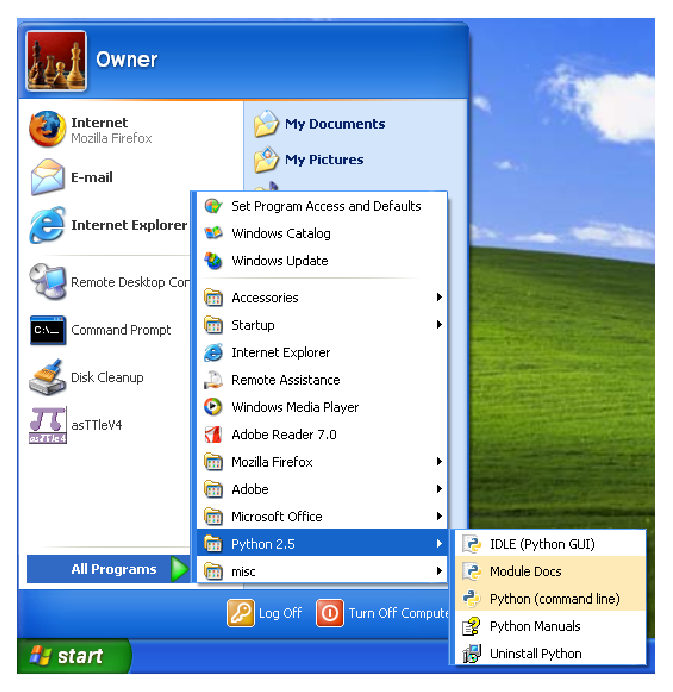
\includegraphics[width=80mm]{eps/figure1.eps}
\end{center}
\caption{Python in the Windows menu.}\label{fig1}
\end{figure}

\begin{figure}
\begin{center}
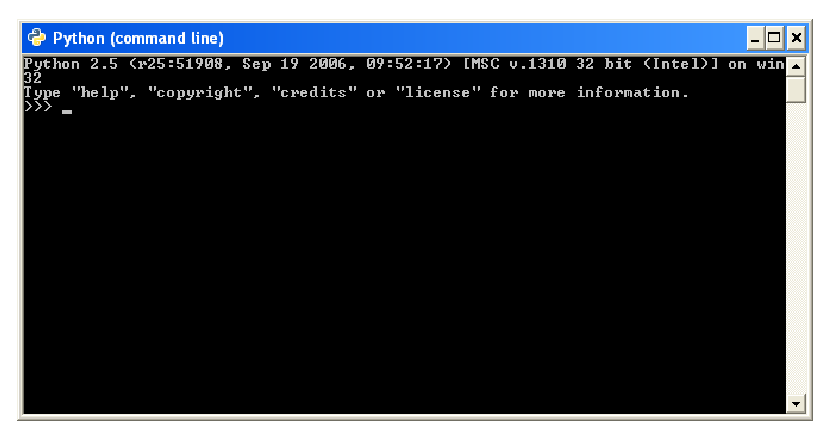
\includegraphics[width=135mm]{eps/figure2.eps}
\end{center}
\caption{The Python console on Windows.}\label{fig2}
\end{figure}
\end{WINDOWS}

\begin{MAC}
In Finder, on the left you should see a group called `Applications'.  Click on this, and then find a program called `Terminal' (it'll probably be in a folder called `Utilities').
Click on `Terminal', and when it starts up, type python and hit enter.  You'll should hopefully be looking at a window that looks like Figure~\ref{fig3}.

\begin{figure}
\begin{center}
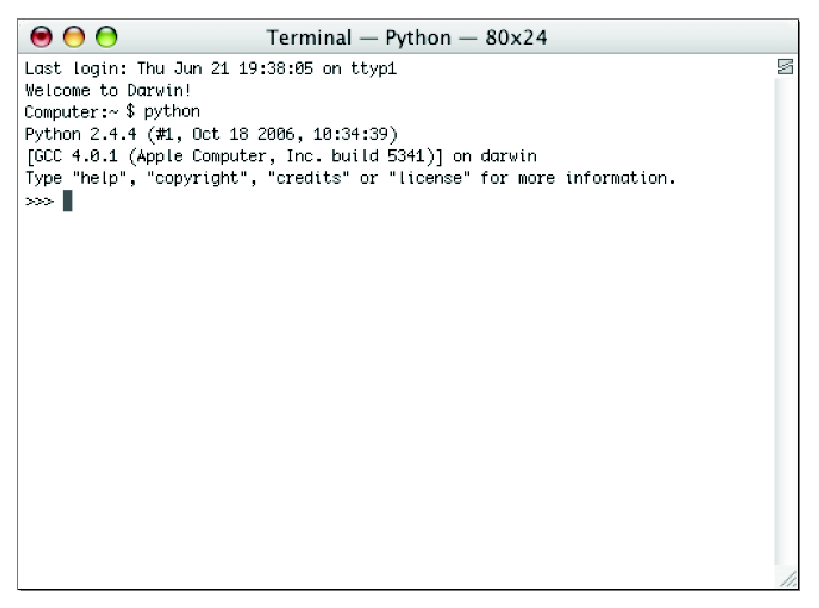
\includegraphics[width=85mm]{eps/figure3.eps}
\end{center}
\caption{The Python console on Mac OSX.}\label{fig3}
\end{figure}
\end{MAC}

\begin{LINUX}
Ask Mum or Dad which terminal application you should use (it could be one called `Konsole', `rxvt', `xterm' or any one of a dozen different programs---which is why you'll probably need to ask).  Start the terminal program and type `python' (without the quotes), and hit enter.  You should see something like Figure~\ref{fig4}.

\begin{figure}
\begin{center}
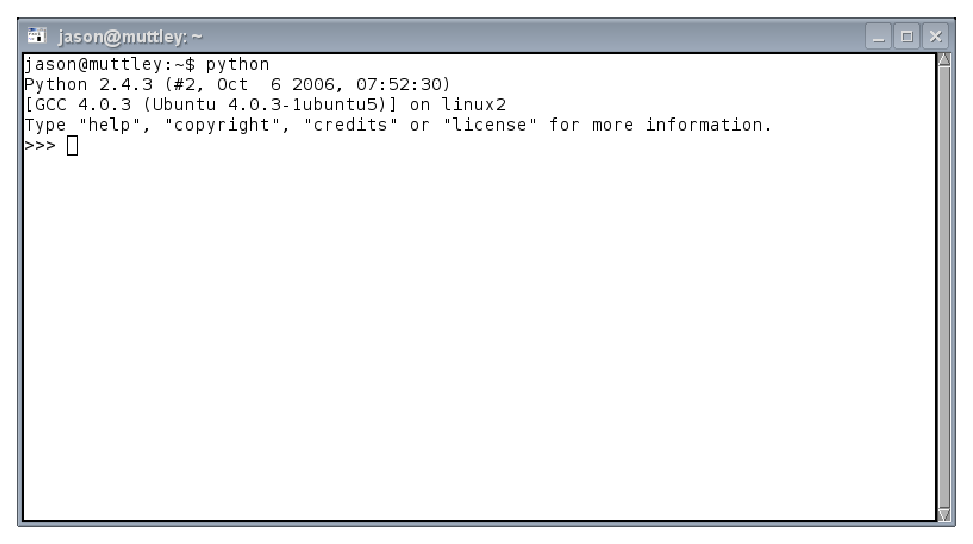
\includegraphics[width=80mm]{eps/figure4.eps}
\end{center}
\caption{The Python console on Linux.}\label{fig4}
\end{figure}
\end{LINUX}

\subsection*{\color{BrickRed}If you discover they haven't read the section in the beginning$\ldots$}

$\ldots$because there is something missing when you try to follow those instructions---then turn to the front of the book, poke it under their nose while they're trying to read the newspaper, and look hopeful.  Saying, ``please please please please'' over and over again, until it becomes annoying, might work quite well, if you're having trouble convincing them to get off the couch.  Of course, the other thing you can do, is turn to the front of the book, and follow the instructions in the Preface to install Python yourself.

\section{Your first Python program}

With any luck, if you've reached this point, you've managed to start up the Python console, which is one way of running Python commands and programs.  When you first start the console (or after entering a command), you'll see what's called a `prompt'.  In the Python console\index{Python console}, the prompt is three chevrons, or greater-than symbols ($>$) pointing to the right:

\begin{listing}
\begin{verbatim}
>>>
\end{verbatim}
\end{listing}

If you put enough Python commands together, you have a program that you can run in more than just the console$\ldots$ but for the moment we're going to keep things simple, and type our commands directly in the console, at the prompt ($>>>$).  So, why not start with typing the following:

\begin{listing}
\begin{verbatim}
print("Hello World")
\end{verbatim}
\end{listing}

Make sure you include the quotes (that's these: $"$ $"$), and hit enter at the end of the line.  Hopefully you'll see something like the following:

\begin{listing}
\begin{verbatim}
>>> print("Hello World")
Hello World
\end{verbatim}
\end{listing}

The prompt reappears, to let you know that the Python console is ready to accept more commands.

\noindent
Congratulations! You've just created your first Python program.  \code{print} is a function that writes whatever is inside the brackets out to the console--we'll use it more later.

\section{Your Second Python program$\ldots$the same again?}

Python programs wouldn't be all that useful if you had to type the commands every single time you wanted to do something---or if you wrote a program for someone, and they had to type it in before they could use it.

The Word Processor that you might be using to write your school assignments, is probably somewhere between 10 and 100 million lines of code.  Depending upon how many lines you printed on one page (and whether or not you printed on both sides of the paper), this could be around 400,000 printed pages$\ldots$ or a stack of paper about 40 metres high.
Just imagine when you brought that software home from the shop, there would be quite a few trips back and forth to the car, to carry that much paper$\ldots$

$\ldots$and you'd better hope there's no big gust of wind while you're carrying those stacks. Luckily, there's an alternative to all this typing---or no one would get anything done.

\begin{center}
\includegraphics*[width=85mm]{eps/pullinghair.eps}
\end{center}

\begin{WINDOWS}
Open Notepad (Click on Start, All Programs, and it should be in the Accessories sub menu), and then type the print command exactly as you typed it into the console before:

\begin{listing}
\begin{verbatim}
print("Hello World")
\end{verbatim}
\end{listing}

Click on the File menu (in Notepad), then Save, and when prompted for a file name, call it \emph{hello.py} and save it on your Desktop. Double-click on the icon for hello.py on your Desktop (see Figure~\ref{fig5}) and for a brief moment a console window will appear.  It will vanish too quickly for you too make out the words, but Hello World will have been printed to the screen for a fraction of a second---we'll come back to this later and prove that it did.\\

\begin{figure}
\begin{center}
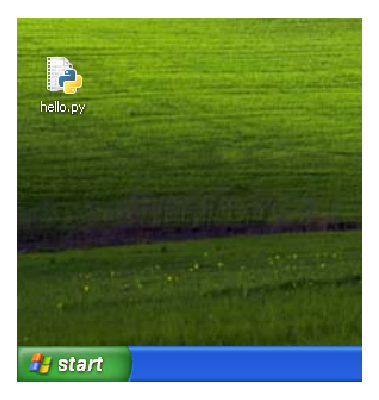
\includegraphics[width=58mm]{eps/figure5.eps}
\end{center}
\caption{hello.py icon on the Windows Desktop.}\label{fig5}
\end{figure}
\end{WINDOWS}

\begin{MAC}
Open up the Text Editor by clicking on its icon.  It may be in the Dock at the bottom of the screen \includegraphics*[width=12mm]{eps/textedit-icon.eps}, or look for this icon \includegraphics*[width=19mm]{eps/textedit-icon2.eps} in the Applications list in Finder.  Type the print command exactly as you typed it into the console earlier:

\begin{listing}
\begin{verbatim}
print("Hello World")
\end{verbatim}
\end{listing}

Click on the File menu, then click on Save, and when you are prompted for a file name, call it hello.py and save it into your home directory (your home directory is on the left under Places--ask Mum or Dad to point it out for you).

Open the `Terminal' application again--it will automatically start up in your home directory--and type the following:

\begin{listing}
\begin{verbatim}
python hello.py
\end{verbatim}
\end{listing}

You should see Hello World written to the window exactly as it was when you typed the command in the Python console.

\end{MAC}

\begin{LINUX}
Open a text editor (again you might have to ask Mum or Dad which one to use), then type the print command exactly as you typed it into the console:

\begin{listing}
\begin{verbatim}
print("Hello World")
\end{verbatim}
\end{listing}

Click on the File menu, then Save, and when prompted for a file name, call it hello.py and save it in your Home folder (there might be an icon called `Home' somewhere in the Save dialog box).  Next open up the terminal application (again Konsole, rxvt, etc... what we used earlier), and type:

\begin{listing}
\begin{verbatim}
python hello.py
\end{verbatim}
\end{listing}

You should see Hello World written to the window exactly as it was when you typed the command in the Python console (see Figure~\ref{fig9}).

\begin{figure}
\begin{center}
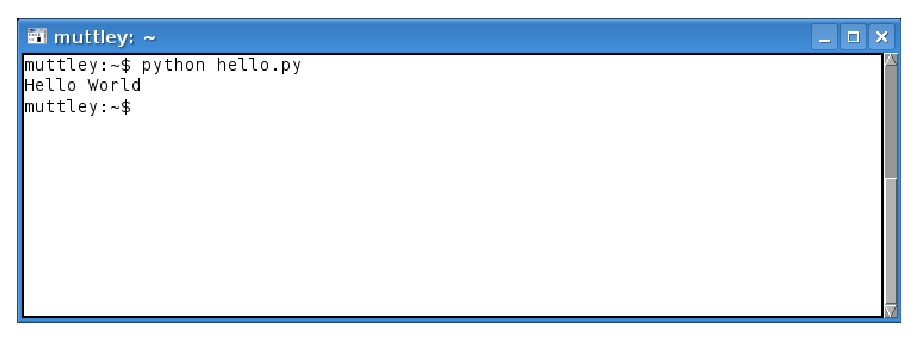
\includegraphics[width=75mm]{eps/figure9.eps}
\end{center}
\caption{Running a python program from a text file on Linux.}\label{fig9}
\end{figure}
\end{LINUX}

So you can now see that the nice people who created Python, have kindly saved you from having to type the same thing over and over and over and over and over again.  Like they did back in the 1980's.  No, I'm serious---they did.  Go and ask your Dad if he ever owned a ZX81 when he was younger?\\

\noindent
If he did you can point at him and laugh.\\

\noindent
Trust me on this one.  You won't get it.  But he will.\footnote{The Sinclair ZX81, released in the 1980's was one of the first affordable home computers.  A number of young boys and girls were driven completely mad, typing in the code for games printed in popular ZX81 magazines---only to discover, after hours of typing, that the darn things never worked properly.}

\noindent
\emph{Be prepared to run away though.}

\subsection*{\color{BrickRed}The End of the Beginning}

Welcome to the wonderful world of Programming.  We've started really simply with a ``Hello World'' application---everyone starts with that, when they're learning to program.
In the next chapter we'll start to do some more useful things with the Python console and then look at what goes into making a program.

\newpage
